\documentclass{beamer}  
\usepackage{../slides}
\usepackage{cancel}
\usepackage{appendixnumberbeamer}
\setbeameroption{hide notes}
\defbeamertemplate{description item}{align left}{\insertdescriptionitem\hfill}

%%%%%%%%%%%%%%%%%%%% Not needed at home!
\usepackage[compatibility=false]{caption}
\usepackage{subcaption}
%%%%%%%%%%%%%%%%%%%% Not needed at home!


\title[Binary Regressors]{Mis-Classified, Binary, Endogenous Regressors: Identification and Inference}
\author[FJ DiTraglia]{Francis J.\ DiTraglia\\ Camilo Garc\'{i}a-Jimeno}
\institute{University of Pennsylvania}
\date{September 14th, 2017}
\begin{document} 
%%%%%%%%%%%%%%%%%%%%%%%%%%%%%%%%%%%%%%%%

\begin{frame}[plain]
	\titlepage 
\end{frame} 
%%%%%%%%%%%%%%%%%%%%%%%%%%%%%%%%%%%%%%%%%
\begin{frame}
  \frametitle{Additively Separable Model}
\[
  y = h(T^*, \mathbf{x}) + \varepsilon
\]
\vspace{-1em}
    \begin{itemize}    
    \item $y$ -- Outcome of interest
    \item $h$ -- Known or unknown function 
    \item $T^*$ -- Unobserved, endogenous binary regressor
    \item $T$ -- Observed, mis-measured binary surrogate for $T^*$
    \item $\mathbf{x}$ -- Exogenous covariates
    \item $\varepsilon$ -- Mean-zero error term
    %\item $z$ -- Discrete (typically binary) instrumental variable
  \end{itemize}

\end{frame}
%%%%%%%%%%%%%%%%%%%%%%%%%%%%%%%%%%%%%%%%%
\begin{frame}
  \frametitle{What is the Effect of $T^*$?}
 
  \begin{block}{Re-write the Model}
\begin{align*}
  y &= c(\mathbf{x}) + \beta(\mathbf{x}) T^* + \varepsilon\\
  &\beta(\mathbf{x}) = h(1,\mathbf{x}) - h(0,\mathbf{x})\\
  &c(\mathbf{x}) = h(0,\mathbf{x})
\end{align*}
  \end{block}

  \begin{alertblock}{This Paper:}
    \begin{itemize}
      \item Does a discrete instrument $z$ (typically binary) identify $\beta(\mathbf{x})$? 
      \item What assumptions are required for $z$ and the surrogate $T$?
      \item How to carry out inference for a mis-classified regressor?
    \end{itemize}
  \end{alertblock}
\end{frame}
%%%%%%%%%%%%%%%%%%%%%%%%%%%%%%%%%%%%%%%%%
\begin{frame}
  \frametitle{Example: Job Training Partnership Act (JTPA)}
\framesubtitle{Heckman et al.\ (2000, QJE)}
Randomized offer of job training, but about $30\%$ of those \emph{not} offered also obtain training and about $40\%$ of those offered training don't attend. Estimate causal effect of \emph{training} rather than \emph{offer} of training.

\begin{itemize}
  \item $y$ -- Log wage 
  \item $T^*$ -- True training attendence
  \item $T$ -- Self-reported training attendance
  \item $\mathbf{x}$ -- Individual characteristics
  \item $z$ -- Offer of job training
\end{itemize}
   
\end{frame}
%%%%%%%%%%%%%%%%%%%%%%%%%%%%%%%%%%%%%%%%%%%%
%\begin{frame}
%  \frametitle{Example: Smoking and Birthweight (SNAP Trial)}
%\framesubtitle{Coleman et al.\ (N Engl J Med, 2012)}
%  RCT with 1050 pregnant smokers in England: 521 given nicotine patches, the rest given placebo patches.
%\begin{itemize}
%  \item $y$ -- Birthweight 
%  \item $T^*$ -- True smoking behavior 
%  \item $T$ -- Self-reported smoking behavior
%  \item $\mathbf{x}$ -- Mother characteristics
%  \item $z$ -- Indicator of nicotine patch
%\end{itemize}
%\end{frame}
%%%%%%%%%%%%%%%%%%%%%%%%%%%%%%%%%%%%%%%%%
%\begin{frame}
%  \frametitle{Example: Schooling and Test Scores}
%\framesubtitle{Burde \& Linden (2013, AEJ Applied)}
%  RCT in Afghanistan: 32 villages divided into 11 clusters. Randomly choose 6 and set up school in each village of these clusters.
%
%\begin{itemize}
%  \item $y$ -- Girl's score on math and language test 
%  \item $T^*$ -- Girl's true school attendance
%  \item $T$ -- Parent's report of child's school attendance
%  \item $\mathbf{x}$ -- Child and household characteristics
%  \item $z$ -- School built in village
%\end{itemize}
%\end{frame}
%%%%%%%%%%%%%%%%%%%%%%%%%%%%%%%%%%%%%%%%%%%
%\begin{frame}
%  \frametitle{Example: Returns to Schooling} 
%\framesubtitle{Oreopoulos (2006, AER)}
%Fuzzy RD: minimum school-leaving age in UK increased from 14 to 15 in 1947 but some already stayed until 15 before the law and others failed to comply after it.
%\begin{itemize}
%  \item $y$ -- Log wage 
%  \item $T^*$ -- School attendance at age 15
%  \item $T$ -- Self-report of school attendance at age 15
%  \item $\mathbf{x}$ -- Individual characteristics
%  \item $z$ -- Indicator: born in or after 1933
%\end{itemize}
%   
%\end{frame}
%%%%%%%%%%%%%%%%%%%%%%%%%%%%%%%%%%%%%%%%%%%
\begin{frame}[label=MAHAJAN_BODY]
  \frametitle{Related Literature}
 
  \begin{block}{Continuous Regressor}
    \small
  Lewbel (1997, 2012), Schennach (2004, 2007), Chen et al. (2005), Hu \& Schennach (2008), Song (2015), Hu et al.\ (2015)\ldots 
  \end{block}

  \begin{block}{Binary, Exogenous Regressor}
    \small
   Aigner (1973), Bollinger (1996), Kane et al. (1999), Black et al. (2000), Frazis \& Loewenstein (2003), Mahajan (2006), Lewbel (2007), Hu (2008)
  \end{block}

  \begin{block}{Binary, Endogenous Regressor}
    \alert{Mahajan (2006)}, \small Shiu (2015), Ura (2015), Denteh et al.\ (2016)  
  \end{block}
\end{frame}
%%%%%%%%%%%%%%%%%%%%%%%%%%%%%%%%%%%%%%%
\begin{frame}
  \frametitle{``Baseline'' Assumptions I -- Model \& Instrument}

  \begin{block}{Additively Separable Model}
    $y = c(\mathbf{x}) + \beta(\mathbf{x}) T^* + \varepsilon, \quad \mathbb{E}[ \varepsilon] = 0$ 
  \end{block}

  \begin{block}{Valid \& Relevant Instrument: $z \in \left\{ 0,1 \right\}$}
    \begin{itemize}
      \item $\mathbb{P}(T^*=1|\mathbf{x},z=1) \neq \mathbb{P}(T^*=1|\mathbf{x},z=0)$
      \item $\mathbb{E}[\varepsilon|\mathbf{x},z] = 0$
      \item $0 < \mathbb{P}(z=1|\mathbf{x}) < 1$
    \end{itemize}
  \end{block}

  \begin{alertblock}{If $T^*$ were observed, these conditions would identify $\beta$\dots}
  \end{alertblock}
\end{frame}
%%%%%%%%%%%%%%%%%%%%%%%%%%%%%%%%%%%%%%%
\begin{frame}
  \frametitle{``Baseline'' Assumptions II -- Measurement Error}


  \begin{alertblock}{Mis-classification Error Rates: ``Truth'' = Subscript}
    \begin{itemize}
      \item[``$\boldsymbol{\uparrow}$''] 
    $\alpha_0(\mathbf{x},z) \equiv \mathbb{P}\left(T=1|T^*=0,\mathbf{x},z  \right)$
  \item[``$\boldsymbol{\downarrow}$''] 
  $\alpha_1(\mathbf{x},z) \equiv \mathbb{P}\left(T=0|T^*=1,\mathbf{x},z  \right)$
    \end{itemize}
  \end{alertblock}

  \begin{block}{Mis-classification unaffected by $z$}
    $\alpha_0(\mathbf{x},z) = \alpha_0(\mathbf{x}), \quad   \alpha_1(\mathbf{x},z) = \alpha_1(\mathbf{x})$
  \end{block}

  \begin{block}{Extent of Mis-classification}
      $\alpha_0(\mathbf{x}) + \alpha_1(\mathbf{x}) < 1 \quad$ ($T$ is positively correlated with $T^*$)
  \end{block}

  \begin{block}{Non-differential Mis-classification}
     $\mathbb{E}[\varepsilon|\mathbf{x},z,T^*,T] = \mathbb{E}[\varepsilon|\mathbf{x},z, T^*]$
  \end{block}



\end{frame}
%%%%%%%%%%%%%%%%%%%%%%%%%%%%%%%%%%%%%%%
\begin{frame}
  \frametitle{Identification Results from the Literature}

  \begin{block}{Mahajan (2006) Theorem 1, Frazis \& Loewenstein (2003)}
    $\mathbb{E}[\varepsilon|\mathbf{x},z,T^*] = 0$, plus ``Baseline'' $\implies \beta(\mathbf{x})$ identified\\
   \hfill \alert{Requires $(T^*,z)$ jointly exogenous.}
  \end{block}

  \begin{block}{Mahajan (2006) A.2}
    $\mathbb{E}[\varepsilon|\mathbf{x}, z, T^*, T] = \mathbb{E}[\varepsilon|\mathbf{x},T^*]$, plus ``Baseline'' $\implies \beta(\mathbf{x})$ identified\\
    \hfill \alert{Allows $T^*$ endogenous, but we prove this claim is false.}
  \end{block}


\end{frame}
%%%%%%%%%%%%%%%%%%%%%%%%%%%%%%%%%%%%%%%
\begin{frame}
  \frametitle{First-stage Probabilities} 

  \begin{table}[h]
    \centering
  \begin{tabular}[h]{|c|c|}
    \hline
   Unobserved & Observed \\
    $p^*_k(\mathbf{x}) \equiv \mathbb{P}(T^*=1|\mathbf{x}, z=k)$ & 
    $p_k(\mathbf{x}) \equiv \mathbb{P}(T=1|\mathbf{x}, z=k)$\\
    \hline
  \end{tabular}
\end{table}


  \begin{block}{Relationship}
    \vspace{-1em}
   \[
     p_k^*(\mathbf{x}) = \frac{p_k(\mathbf{x}) - \alpha_0(\mathbf{x})}{1 - \alpha_0(\mathbf{x}) - \alpha_1(\mathbf{x})}, \quad k = 0,1
   \]
   \hfill\alert{\footnotesize $z$ does not affect $(\alpha_0, \alpha_1)$; denominator $\neq 0$}
  \end{block}

  \normalsize
  \begin{block}{Bounds for Mis-classification}
    \vspace{-1em}
    \[
      \alpha_0(\mathbf{x}) \leq p_k(\mathbf{x}) \leq 1 - \alpha_1(\mathbf{x}), \quad k = 0,1
    \]
   \hfill \alert{\footnotesize$\alpha_0(\mathbf{x}) + \alpha_1(\mathbf{x}) <1$}
  \end{block}

\end{frame}
%%%%%%%%%%%%%%%%%%%%%%%%%%%%%%%%%%%%%%%
\begin{frame}[plain, c]
  \frametitle{$\alpha_0 \leq \min_k \left\{p_k\right\}, \; \; \alpha_1 \leq \min_k \left\{1 - p_k\right\}$}
\begin{figure}[h]
  \centering
  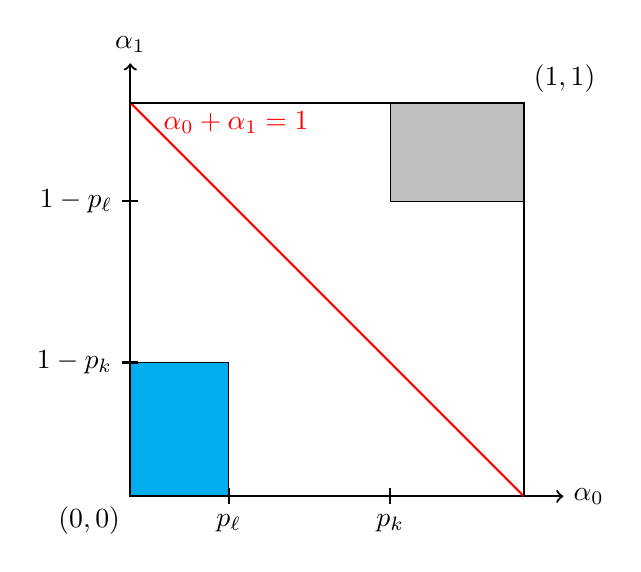
\begin{tikzpicture}[scale=5]
    \draw [fill = lightgray] (0.66,0.75) rectangle (1,1);
    \draw [fill = cyan] (0,0) rectangle (0.25, 0.34);
    \draw [thick, <->] (0,1.1)
    node[above] {$\alpha_1$} -- (0,0) 
    node [below left] {$(0,0)$} -- (1.1,0) 
    node [right] {$\alpha_0$};
    \draw [thick] (0.25,0.02) -- (0.25,-0.02) node [below] {$p_\ell$}; 
    \draw [thick] (0.02,0.75) -- (-0.02,0.75) node [left] {$1 - p_\ell$}; 
    \draw [thick] (0.66,0.02) -- (0.66,-0.02) node [below] {$p_k$}; 
    \draw [thick] (0.02,0.34) -- (-0.02,0.34) node [left] {$1 - p_k$}; 
    \draw [thick, red] (0,1) to (1,0); 
    \node [right, red] at (0.06,0.95) {$\alpha_0 + \alpha_1 = 1$};
    \draw [thick] (0,1) -- (1,1) -- (1,0);
    \node [above right] at (1,1) {$(1,1)$};
    \end{tikzpicture}
\end{figure}
\end{frame}
%%%%%%%%%%%%%%%%%%%%%%%%%%%%%%%%%%%%%%
\begin{frame}
  \frametitle{Instrumental Variable (Wald) Estimands}
  \begin{block}{Unobserved}
  \[
    \beta(\mathbf{x}) = \frac{\mathbb{E}[y|\mathbf{x},z=1] - \mathbb{E}[y|\mathbf{x},z=0]}{p^*_1(\mathbf{x}) - p^*_0(\mathbf{x})} 
  \]
  \end{block}

  \begin{block}{Observed}
    \vspace{-1em}
    \small
    \[
      \frac{\mathbb{E}[y|\mathbf{x},z=1] - \mathbb{E}[y|\mathbf{x},z=0]}{p_1(\mathbf{x}) - p_0(\mathbf{x})} = \beta(\mathbf{x})\left[ \frac{p_1^*(\mathbf{x}) - p_0^*(\mathbf{x})}{p_1(\mathbf{x}) - p_0(\mathbf{x})} \right] = \alert{\frac{\beta(\mathbf{x})}{1 - \alpha_0(\mathbf{x}) - \alpha_1(\mathbf{x})} }
    \]
   
    \vspace{2em}
    \scriptsize
    \[
      \boxed{p_1^*(\mathbf{x}) - p_0^*(\mathbf{x}) = \frac{p_1(\mathbf{x}) - \alpha_0(\mathbf{x})}{1 - \alpha_0 - \alpha_1(\mathbf{x})} -   \frac{p_0(\mathbf{x}) - \alpha_0(\mathbf{x})}{1 - \alpha_0 - \alpha_1(\mathbf{x})} = \frac{p_1(\mathbf{x}) - p_0(\mathbf{x})}{1 - \alpha_0(\mathbf{x}) - \alpha_1(\mathbf{x})}}
    \]
  \end{block}
\end{frame}
%%%%%%%%%%%%%%%%%%%%%%%%%%%%%%%%%%%%%%
\begin{frame}
  \frametitle{Partial Identification Bounds for $\beta(\mathbf{x})$}

    \footnotesize
    \[
      \boxed{ \beta(\mathbf{x}) = \left[ 1 - \alpha_0(\mathbf{x}) - \alpha_1(\mathbf{x}) \right] 
     \left[\frac{\mathbb{E}\left[y|\mathbf{x},z=1\right] - \mathbb{E}\left[y|\mathbf{x},z=0\right]}{p_1(\mathbf{x}) - p_0(\mathbf{x})}\right] }
    \]

    \footnotesize
    \[
      \boxed{ 0 \leq \alpha_0 \leq \min_k \{p_k(\mathbf{x})\}, \quad 0 \leq \alpha_1 \leq \min_k \{1 - p_k(\mathbf{x})\}}
    \]

    \normalsize
    \begin{block}{No Mis-classification}
      $\alpha_0(\mathbf{x}) =  \alpha_1(\mathbf{x}) = 0 \implies \alert{\beta(\mathbf{x}) = }$ \alert{Observed Wald Estimand}
    \end{block}

    \begin{block}{Maximum Mis-classification}
      $\alpha_0(\mathbf{x}) = p_{\min}(\mathbf{x}), \, \alpha_1(\mathbf{x}) = 1 - p_{\max}(\mathbf{x})$

      \vspace{-0.5em}
      \begin{align*}
        \implies 1 - \alpha_0(\mathbf{x}) - \alpha_1(\mathbf{x}) = p_{\max}(\mathbf{x}) - p_{\min}(\mathbf{x})
      = |p_1(\mathbf{x}) - p_0(\mathbf{x})|\\
      \implies \alert{\beta(\mathbf{x}) =\mbox{sign}\left\{ p_1(\mathbf{x}) - p_0(\mathbf{x}) \right\}\times (\mbox{Reduced Form})}
    \end{align*}
      
    \end{block}
  
\end{frame}
%%%%%%%%%%%%%%%%%%%%%%%%%%%%%%%%%%%%%%
\begin{frame}
  \frametitle{Partial Identification Bounds for $\beta(\mathbf{x})$}

    \begin{block}{No Mis-classification}
      $\beta(\mathbf{x}) = $ Observed Wald Estimand
    \end{block}

    \begin{block}{Maximum Mis-classification}
      \vspace{-1.5em}
      \begin{align*}
        \beta(\mathbf{x}) &=\mbox{sign}\left\{ p_1(\mathbf{x}) - p_0(\mathbf{x}) \right\}\times (\mbox{Reduced Form})\\
        &=\mbox{sign}\left\{ \mbox{Observed Wald} \right\} \times |\mbox{Reduced Form}|
      \end{align*}
      
      \vspace{1em}
    \footnotesize Observed Wald $> 0\iff \mbox{sign}\left\{ p_1(\mathbf{x}) - p_0(\mathbf{x}) \right\} = \mbox{sign}\left\{ \mbox{Reduced Form} \right\}$ \\
    \footnotesize Observed Wald $< 0\iff \mbox{sign}\left\{ p_1(\mathbf{x}) - p_0(\mathbf{x}) \right\} \neq \mbox{sign}\left\{ \mbox{Reduced Form} \right\}$ 
    \end{block}

    \vspace{1em}
    \begin{alertblock}{
        $\beta(\mathbf{x})$ has the same sign as the observed Wald and its magnitude is between that of Wald and Reduced Form.}
    \end{alertblock}

\end{frame}
%%%%%%%%%%%%%%%%%%%%%%%%%%%%%%%%%%%%%%
\begin{frame}
  \frametitle{Sharp Bounds?}

  \begin{itemize}
    \item Bounds from the preceding slide are known in the literature.
    \item We prove that they are \emph{not} sharp under the baseline assumptions from above.
      \item $\mathbb{E}[\varepsilon|\mathbf{x},T^*,T,z] = \mathbb{E}[\varepsilon|\mathbf{x},T^*,z]$ restricts $(\alpha_0,\alpha_1)$ hence $\beta$.
    \item Description of the sharp set is somewhat complicated\dots
    \item Corollary: $\beta$ is not point identified regardless of how many (discrete) values $z$ takes on.
  \end{itemize}

  \begin{alertblock}{Point identification from slightly stronger assumptions?}
  \end{alertblock}

\end{frame}
%%%%%%%%%%%%%%%%%%%%%%%%%%%%%%%%%%%%%%
\begin{frame}
  \frametitle{Point Identification: Part I}


  \vspace{-1em}

  \begin{block}{Reparameterization}
    \vspace{-1em}
\begin{align*}
  \theta_1(\mathbf{x}) &= \beta(\mathbf{x})/\left[ 1 - \alpha_0(\mathbf{x}) - \mathbf{\alpha}_1(\mathbf{x})  \right]\\
  \theta_2(\mathbf{x}) &= \left[\theta_1(\mathbf{x})\right]^2 \left[ 1 + \alpha_0(\mathbf{x}) - \alpha_1(\mathbf{x})\right] \\
  \theta_3(\mathbf{x}) &= \left[\theta_1(\mathbf{x})\right]^3\left[ \left\{ 1 - \alpha_0(\mathbf{x}) - \alpha_1(\mathbf{x}) \right\}^2 + 6\alpha_0(\mathbf{x})\left\{ 1 - \alpha_1(\mathbf{x}) \right\} \right]
\end{align*}

\[\boxed{\beta(\mathbf{x}) = 0 \iff \theta_1(\mathbf{x}) = \theta_2(\mathbf{x}) = \theta_3(\mathbf{x}) = 0}\]
  \end{block}

  \vspace{-1.5em}

  \begin{block}{Lemma}
    Baseline Assumptions $\implies \mbox{Cov}(y,z|\mathbf{x}) - \theta_1(\mathbf{x}) \mbox{Cov}(z,T|\mathbf{x}) = 0$.
  \end{block}

\end{frame}
%%%%%%%%%%%%%%%%%%%%%%%%%%%%%%%%%%%%%%
\begin{frame}
  \frametitle{Point Identification: Part II}

  \begin{block}{Assumption (\spadesuit)}
    $\mathbb{E}[\varepsilon^2|\mathbf{x},z] = \mathbb{E}[\varepsilon^2|\mathbf{x}]$
  \end{block}

  \begin{block}{Lemma}
    (Baseline) + (\spadesuit) $\implies$ 
    \[
      \alert{\mbox{Cov}(y^2,z|\mathbf{x}) = 2\mbox{Cov}(yT,z|\mathbf{x}) \theta_1(\mathbf{x}) -\mbox{Cov}(T,z|\mathbf{x})\theta_2(\mathbf{x})}
    \]
  \end{block}

  \begin{block}{Corollary}
    (Baseline) + (\spadesuit) + $[\beta(\mathbf{x})\neq 0] \implies \left[ \alpha_1(\mathbf{x}) - \alpha_0(\mathbf{x}) \right]$ is identified. Hence, $\beta(\mathbf{x})$ is identified if mis-classification is one-sided.
  \end{block}
    

  
\end{frame}
%%%%%%%%%%%%%%%%%%%%%%%%%%%%%%%%%%%%%%
\begin{frame}
  \frametitle{Point Identification: Part III}

  \begin{block}{Assumption (\clubsuit)}
    \begin{enumerate}[(i)]
    \item $\mathbb{E}[\varepsilon^2|\mathbf{x},z,T^*,T] = \mathbb{E}[\varepsilon^2|\mathbf{x},z, T^*]$
    \item $\mathbb{E}[\varepsilon^3|\mathbf{x},z] = \mathbb{E}[\varepsilon^3|\mathbf{x}]$
  \end{enumerate}
  \end{block}
  
\end{frame}
%%%%%%%%%%%%%%%%%%%%%%%%%%%%%%%%%%%%%%
\begin{frame}
  \begin{alertblock}{Sufficient Conditions for (\spadesuit) and (\clubsuit)}
    \begin{enumerate}[(i)]
      \item $T$ is conditionally independent of $(\varepsilon,z)$ given $(T^*,\mathbf{x})$
      \item $z$ is conditionally independent of $\varepsilon$ given $\mathbf{x}$
    \end{enumerate}
  \end{alertblock}
  
\end{frame}
%%%%%%%%%%%%%%%%%%%%%%%%%%%%%%%%%%%%%%
\begin{frame}
  \frametitle{Identification Argument: Step I}
 
  \begin{block}{Reparameterization}
    \vspace{-1em}
\begin{align*}
  \theta_1(\mathbf{x}) &= \beta(\mathbf{x})/\left[ 1 - \alpha_0(\mathbf{x}) - \mathbf{\alpha}_1(\mathbf{x})  \right]\\
  \theta_2(\mathbf{x}) &= \left[\theta_1(\mathbf{x})\right]^2 \left[ 1 + \alpha_0(\mathbf{x}) - \alpha_1(\mathbf{x})\right] \\
  \theta_3(\mathbf{x}) &= \left[\theta_1(\mathbf{x})\right]^3\left[ \left\{ 1 - \alpha_0(\mathbf{x}) - \alpha_1(\mathbf{x}) \right\}^2 + 6\alpha_0(\mathbf{x})\left\{ 1 - \alpha_1(\mathbf{x}) \right\} \right]
\end{align*}
  \end{block}

  \begin{alertblock}{Theorem}
    If $\theta_1(\mathbf{x}), \theta_2(\mathbf{x})$ and $\theta_3(\mathbf{x})$ are identified and $\alpha_0(\mathbf{x}) + \alpha_1(\mathbf{x}) <1$
    \begin{itemize}
      \item If $\theta_1(\mathbf{x})\neq 0$, then $\beta(\mathbf{x}), \alpha_0(\mathbf{x})$ and $\alpha_1(\mathbf{x})$ are identified 
      \item If $\theta_1(\mathbf{x}) = 0$ then $\beta(\mathbf{x})$ is identified %but $\alpha_0(\mathbf{x})$ and $\mathbf{\alpha}_1(\mathbf{x})$ are not.
    \end{itemize}
    If $\alpha_0(\mathbf{x}) + \alpha_1(\mathbf{x}) \neq 1$,  then $\beta(\mathbf{x})$ is identified up to sign.
  \end{alertblock}
  
\end{frame}
%%%%%%%%%%%%%%%%%%%%%%%%%%%%%%%%%%%%%%
\begin{frame}
  \frametitle{Identification Argument: Step II}

  \begin{block}{Notation}
    \vspace{-1em}
\[
    \pi(\mathbf{x}) = \mbox{Cov}(T,z|\mathbf{x}), \quad \eta_j(\mathbf{x}) = \mbox{Cov}(y^j,z|\mathbf{x}), \quad \tau_j(\mathbf{x}) = \mbox{Cov}(Ty^j,z|\mathbf{x})
\]
  \end{block}

  \begin{alertblock}{Theorem} 
    Baseline plus 2nd and 3rd Moment Assumptions imply 
\begin{align*}
 \eta_1(\mathbf{x}) &= \pi(\mathbf{x})\theta_1(\mathbf{x})\\
  \eta_2(\mathbf{x}) &=  2\tau_1(\mathbf{x}) \theta_1(\mathbf{x}) - \pi(\mathbf{x})\theta_2(\mathbf{x}) \\
  \eta_3(\mathbf{x}) &=  3\tau_2(\mathbf{x}) \theta_1(\mathbf{x}) - 3\tau_1(\mathbf{x}) \theta_2(\mathbf{x}) + \pi(\mathbf{x})\theta_3(\mathbf{x})
\end{align*}
so $\theta_1(\mathbf{x}), \theta_2(\mathbf{x})$ and $\theta_3(\mathbf{x})$ are identified if $\pi(\mathbf{x})\neq 0$.
  \end{alertblock}



\end{frame}
%%%%%%%%%%%%%%%%%%%%%%%%%%%%%%%%%%%%%%
%\begin{frame}
%  \frametitle{Some Intuition: Suppress Dependence on Covariates} 
%
%  \begin{block}{Baseline Assumptions}
%    \footnotesize
%    \[\mbox{Cov}(y,z) - \left( \frac{\beta}{1 - \alpha_0 - \alpha_1} \right) \mbox{Cov}(T,z) = 0\]
%    \hfill \alert{Identifies $\beta / (1 - \alpha_0 - \alpha_1)$}
%  \end{block}
%
%  \begin{block}{Second Moment Assumptions}
%    \scriptsize
%    \[\mbox{Cov}(y^2,z) - \frac{\beta}{1 - \alpha_0 - \alpha_1}\left\{2\mbox{Cov}(yT,z)- \left(\frac{\beta}{1 - \alpha_0 - \alpha_1}\right) \mbox{Cov}(T,z)\left(1 + \alpha_0 - \alpha_1\right)  \right\} = 0
%    \]
%
%    \vspace{0.5em}
%
%  \hfill \alert{Given $\beta/(1 - \alpha_0 - \alpha_1)$, identifies $\alpha_0 - \alpha_1$}
%  \end{block}
%
%  \begin{block}{Third Moment Assumptions}
%    \footnotesize
%    Messy, but can be shown yield two quadratics with \alert{identical coefficients}: one in $\alpha_0$ and the other in $1 - \alpha_1$.
%Roots are real provided that $\alpha_0 + \alpha_1 \neq 0$ but to tell which is $\alpha_0$ and which is $1 - \alpha_1$ we require $\alpha_0 + \alpha_1 < 1$.
%\end{block}
%
%\end{frame}
%%%%%%%%%%%%%%%%%%%%%%%%%%%%%%%%%%%%%%
\begin{frame}
  \frametitle{Simple Special Case}


  \begin{block}{Suppose $\alpha_0 = 0$ and No Covariates}
  \begin{align*}
    \mbox{Cov}(y,z) - \left( \frac{\beta}{1 - \alpha_1} \right) \mbox{Cov}(T,z) &= 0\\
      \mbox{Cov}(y^2,z) - \frac{\beta}{1 - \alpha_1}\left\{2\mbox{Cov}(yT,z)- \beta \mbox{Cov}(T,z)\right\} &= 0
  \end{align*}
  \end{block}

  \begin{block}{Closed-Form Solution for $\beta$}
  \[
    \alert{\beta = \frac{2\mbox{Cov}(yT,z)}{\mbox{Cov}(T,z)} - \frac{\mbox{Cov}(y^2,z)}{\mbox{Cov}(y,z)}}
  \]
  \end{block}

\end{frame}
%%%%%%%%%%%%%%%%%%%%%%%%%%%%%%%%%%%%%%
\begin{frame}
  \frametitle{Unconditional Moment Equalities ($\alpha_0 = 0$, No Covariates)}

\[
  \mathbf{u}_i(\boldsymbol{\kappa}, \boldsymbol{\theta}) = \left[
  \begin{array}{l}
  y_i - \kappa_1 - \theta_1 T_i\\
  y^2_i - \kappa_2  - \theta_1 2y_iT_i + \theta_2 T_i
  \end{array}
\right], \quad
 \mathbb{E}
  \left[
  \begin{array}{l}
    \boldsymbol{u}_i(\boldsymbol{\kappa}, \boldsymbol{\theta}) \\ \mathbf{u}_i(\boldsymbol{\kappa}, \boldsymbol{\theta}) z_i
  \end{array}
\right] = \mathbf{0}
\]

\small
\begin{align*}
    \theta_1 &= \beta / (1 - \alpha_1)\\
    \theta_2 &= \beta^2 / (1 - \alpha_1)\\
    \kappa_1 &= c\\
    \kappa_2 &= c^2 + \sigma_{\varepsilon}^2
  \end{align*}

  \alert{What happens if we try standard GMM inference?}

\end{frame}
%%%%%%%%%%%%%%%%%%%%%%%%%%%%%%%%%%%%%%
\begin{frame}
  \frametitle{Simulation DGP: $y = \beta T^* + \varepsilon$}
  \begin{block}{Errors}
      $(\varepsilon, \eta) \sim $ jointly normal, mean 0, variance 1, correlation 0.5.
  \end{block}
  \begin{block}{First-Stage}
      \begin{itemize}
        \item Half of individuals have $z=1$, the rest have $z=0$.
        \item $T^* = \mathbf{1}\left\{ \gamma_0 + \gamma_1 z + \eta > 0 \right\}$
        \item $\delta = \mathbb{P}(T^* = 0|z =1) = \mathbb{P}(T^*=1|z=0) = 0.15$
          %\begin{itemize}
        %\item $\gamma_0 = \Phi^{-1}(\delta)$
        %\item $\gamma_1 = \Phi^{-1}(1-\delta) - \Phi(\delta)$   
      %\end{itemize}
      \end{itemize}
  \end{block}
  \vspace{-1em}


  \begin{block}{Mis-classification}
      \begin{itemize}
        \item Set $\alpha_0 = 0$ 
        \item $T|T^*=1 \sim \mbox{Bernoulli}(1-\alpha_1)$
      \end{itemize}
  \end{block}
  
\end{frame}
%%%%%%%%%%%%%%%%%%%%%%%%%%%%%%%%%%%%%%
\begin{frame}
  \frametitle{Coverage and Width of Nominal 95\% GMM CIs}
  \framesubtitle{$\alpha_1 = 0.1, \delta = 0.15, n = 1000, \rho = 0.5$, 5000 simulation replications}
\begin{table}[!tbp]
  \small
\centering
\begin{tabular}{ccc}
\hline\hline
$\beta$ & Coverage & Median Width \\
\hline
$2.00$&$0.95$&$0.23$\tabularnewline
$1.50$&$0.95$&$0.26$\tabularnewline
$1.00$&$0.95$&$0.32$\tabularnewline
$0.50$&$0.96$&$0.55$\tabularnewline
$0.25$&$0.98$&$1.08$\tabularnewline
$0.20$&$0.99$&$1.40$\tabularnewline
$0.15$&$0.99$&$1.86$\tabularnewline
$0.10$&$1.00$&$3.04$\tabularnewline
$0.05$&$1.00$&$4.76$\tabularnewline
$0.01$&$1.00$&$5.92$\tabularnewline
\hline
\end{tabular}
\end{table}
\end{frame}

%%%%%%%%%%%%%%%%%%%%%%%%%%%%%%%%%%%%%
%\begin{frame}[plain,c]
%
%  \begin{figure}[h]
%    \centering
%    \includegraphics[width=\textwidth]{Rplot1}
%  \end{figure}
%
%\end{frame}
%%%%%%%%%%%%%%%%%%%%%%%%%%%%%%%%%%%%%%
\begin{frame}[plain,c]

  \begin{figure}[h]
    \centering
    %\includegraphics[width=\textwidth]{Rplot2}
  \end{figure}

\end{frame}
%%%%%%%%%%%%%%%%%%%%%%%%%%%%%%%%%%%%%%
\begin{frame}[plain,c]

  \begin{figure}[h]
    \centering
    %\includegraphics[width=\textwidth]{Rplot4}
  \end{figure}

\end{frame}
%%%%%%%%%%%%%%%%%%%%%%%%%%%%%%%%%%%%%%%
\begin{frame}[plain,c]

  \begin{figure}[h]
    \centering
    %\includegraphics[width=\textwidth]{Rplot9}
  \end{figure}

\end{frame}
%%%%%%%%%%%%%%%%%%%%%%%%%%%%%%%%%%%%%%
\begin{frame}
  \frametitle{Weak Identification Problem}
  \framesubtitle{Illustrated for $\alpha_0 = 0$ but holds generally}

  \small
\[
  \mathbf{u}_i(\boldsymbol{\kappa}, \boldsymbol{\theta}) = \left[
  \begin{array}{l}
  y_i - \kappa_1 - \theta_1 T_i\\
  y^2_i - \kappa_2  - \theta_1 2y_iT_i + \theta_2 T_i
  \end{array}
\right], \quad
 \mathbb{E}
  \left[
  \begin{array}{l}
    \boldsymbol{u}_i(\boldsymbol{\kappa}, \boldsymbol{\theta}) \\ \mathbf{u}_i(\boldsymbol{\kappa}, \boldsymbol{\theta}) z_i
  \end{array}
\right] = \mathbf{0}
\]

\[
  \alert{\theta_1 = \beta / (1 - \alpha_1),} \quad
  \alert{\theta_2 = \beta^2 / (1 - \alpha_1)}
\] 

\begin{itemize}
  \item $\beta$ small $\Rightarrow$ moment equalities uninformative about $\alpha_1$
  \item Same problem for other estimators from the literature but hasn't been pointed out.
  \item Identification robust inference: GMM Anderson-Rubin statistic
  \item \alert{But we can do better\ldots}
\end{itemize}


\end{frame}
%%%%%%%%%%%%%%%%%%%%%%%%%%%%%%%%%%%%%%
\begin{frame}
  \frametitle{``Weak'' Bounds for $\alpha_0, \alpha_1$}
  \framesubtitle{General Case $\alpha_0 \neq 0$}

  \small

  \begin{block}{\small Law of Total Probability}
  \[
    p_k^* = \frac{p_k - \alpha_0}{1 - \alpha_0 - \alpha_1}, \quad
  1 - p_k^* = \frac{1 - p_k - \alpha_1}{1 - \alpha_0 - \alpha_1}\]
    where $p_k = \mathbb{P}(T=1|z=k), \quad p^*_k = \mathbb{P}(T^*=1|z=k)$ 
  \end{block}

  \begin{block}{\small $Cor(T,T^*)>0$}
   $\iff \alpha_0 + \alpha_1 < 1 \iff 1 - \alpha_0 - \alpha_1 > 0$ 
  \end{block}



  \begin{alertblock}{Implications}
    \vspace{-1em}
    \begin{itemize}
      \item $\alpha_0 < \min_k \left\{ p_k \right\}, \quad \alpha_1 < \min_k \left\{ 1 - p_k \right\}$
      \item $\beta$ is between $\beta_{RF}$ and $\beta_{IV}$ 
      \item $\beta_{IV}$ \emph{inflated} but has correct sign 
    \end{itemize}
  \end{alertblock}
  
\end{frame}
%%%%%%%%%%%%%%%%%%%%%%%%%%%%%%%%%%%%%%
\begin{frame}
  \frametitle{Second Moment Bounds for $\alpha_0, \alpha_1$}
  \small

  \begin{block}{Observables}
    $\sigma^2_{tk} = \mbox{Var}(y|T=t,z_k), \quad \mu_{tk} = \mathbb{E}[y|T=t, z_k], \quad p_k = \mathbb{P}(T=1|z_k)$
  \end{block}

  \begin{block}{Constraint on Unobservables}
    $\mbox{Var}(\varepsilon|T^*=t, z_k) > 0$ 

    \begin{block}{Equivalent To}
\begin{align*}
  (p_k - \alpha_0) \left[ \left(\frac{1 - \alpha_0}{1 - p_k}\right) \sigma^2_{1k} - \left(\frac{\alpha_0}{p_k}\right) \sigma_{0k}^2 \right] &> \alpha_0 (1 - \alpha_0)(\mu_{1k} - \mu_{0k})^2\\
  (1 - p_k - \alpha_1) \left[ \left(\frac{1 - \alpha_1}{p_k}\right) \sigma^2_{0k} - \left(\frac{\alpha_1}{1-p_k}\right) \sigma_{1k}^2 \right] &> \alpha_1 (1 - \alpha_1)(\mu_{1k} - \mu_{0k})^2
\end{align*}

    \end{block} 
  \end{block}
\end{frame}
%%%%%%%%%%%%%%%%%%%%%%%%%%%%%%%%%%%%%%
\begin{frame}[c]
  \frametitle{Bounds can be very informative in practice\ldots}
  \framesubtitle{Figure based on data from Burde \& Linden (2013)}
\begin{columns}[c]
  \begin{column}{0.4\textwidth}
    \begin{block}{``Weak'' Bounds}
      $\beta \in [0.65 \times\beta_{IV},\; \beta_{IV}]$
    \end{block}
    \vspace{1em}
    \begin{alertblock}{Add 2nd Moments}
      $\beta \in [0.78 \times \beta_{IV},\;\beta_{IV}]$
    \end{alertblock}
  \end{column}
  \begin{column}{0.6\textwidth}
      \begin{figure}[h]
        \centering
        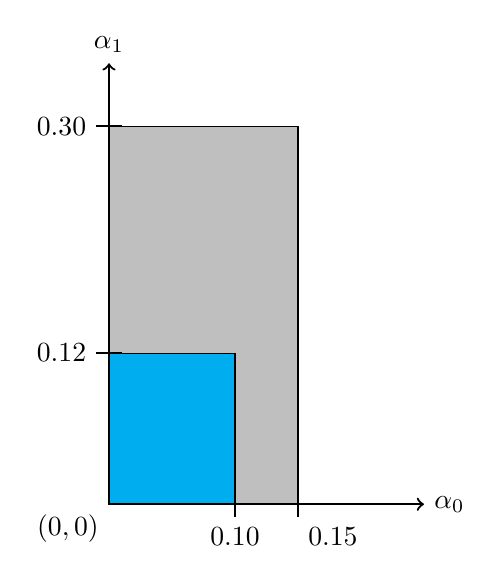
\begin{tikzpicture}[scale=16]
          \draw [fill = lightgray] (0,0) rectangle (0.15, 0.3);
          \draw [fill = cyan] (0,0) rectangle (0.10, 0.12);
          \draw [thick, <->] (0,0.35)
          node[above] {$\alpha_1$} -- (0,0) 
          node [below left] {$(0,0)$} -- (0.25,0) 
          node [right] {$\alpha_0$};
          \draw [thick] (0.15,0.01) -- (0.15,-0.01) node [below right] {$0.15$}; 
          \draw [thick] (0.1,0.01) -- (0.1,-0.01) node [below] {$0.10$}; 
          \draw [thick] (0.01,0.3) -- (-0.01,0.3) node [left] {0.30}; 
          \draw [thick] (0.01,0.12) -- (-0.01,0.12) node [left] {0.12}; 
          \end{tikzpicture}
      \end{figure}
  \end{column}
\end{columns}
 
\end{frame}
%%%%%%%%%%%%%%%%%%%%%%%%%%%%%%%%%%%%%
\begin{frame}
  \frametitle{Adding Auxiliary Moment Inequalities}

  \begin{itemize}
    \item Bounds for $(\alpha_0, \alpha_1)$ immune to weak identification problem: remain informative if $\beta$ is small or zero.
    \item 2nd moment bounds strictly tighter, but still need weak bounds to determine which root of  quadratic is extraneous.
    \item Since $\beta /(1 - \alpha_0 - \alpha_1)$ is identified by TSLS, get meaningful restrictions on $\beta$.
    \item Inference using Generalized Moment Selection (Andrews \& Soares, 2010)
  \end{itemize}

  
\end{frame}
%%%%%%%%%%%%%%%%%%%%%%%%%%%%%%%%%%%%%
\begin{frame}
  \frametitle{Inference With Moment Equalities and Inequalities}
  \small

\begin{block}{Moment Conditions}
  $\mathbb{E} \left[ m_j(\mathbf{w}_i,\theta_0) \right] \geq 0, \quad j = 1, \cdots, p$\\
  $\mathbb{E} \left[ m_j(\mathbf{w}_i,\theta_0) \right]  = 0, \quad j = p+1, \cdots, p + v$
\end{block}


\begin{block}{Test Statistic}
  \vspace{-1em}
\[
  T_n(\theta) = \sum_{j=1}^p \left[\frac{\sqrt{n}\; \bar{m}_{n,j}(\theta)}{\widehat{\sigma}_{n,j}(\theta)}\right]^2_- + \sum_{j=p+1}^{p+v} \left[\frac{\sqrt{n}\; \bar{m}_{n,j}(\theta)}{\widehat{\sigma}_{n,j}(\theta)}\right]^2
\]
\footnotesize
\begin{align*}
[x]_- &= \min\left\{ x, 0 \right\}\\
\bar{m}_{n,j}(\theta) &= n^{-1} \sum_{i=1}^{n} m_j(\mathbf{w}_i, \theta)\\
\widehat{\sigma}^2_{n,j}(\theta) &=  \mbox{consistent est.\ of } \mbox{AVAR}\left[  \sqrt{n}\; \bar{m}_{n,j}(\theta)\right]
\end{align*}
\end{block}

\end{frame}
%%%%%%%%%%%%%%%%%%%%%%%%%%%%%%%%%%%%%
\begin{frame}
  \frametitle{Inference via Generalized Moment Selection}
  \framesubtitle{Andrews \& Soares (2010)}

  \begin{block}{Moment Selection Step}
    If $\displaystyle\frac{\sqrt{n}\,\bar{m}_{n,j}(\theta_0)}{\widehat{\sigma}_{n,j}(\theta_0)} > \sqrt{\ln n}$ then drop inequality $j$
  \end{block}

  \begin{block}{Critical Value} 
    \begin{itemize}
      \item $\sqrt{n}\, \bar{m}_n(\theta_0) \rightarrow_d$ normal limit with covariance matrix $\Sigma(\theta_0)$
      \item Use this to bootstrap the limit distribution of the test statistic.
    \end{itemize}
  \end{block}

  \begin{block}{Theoretical Guarantees}
    Uniformly valid test of $H_0\colon \theta = \theta_0$ \alert{regardless of whether $\theta_0$ is identified}.
    Not asymptotically conservative.
  \end{block}

\end{frame}
%%%%%%%%%%%%%%%%%%%%%%%%%%%%%%%%%%%%%
\begin{frame}
  \frametitle{Confidence Regions}
  \begin{itemize}
    \item Invert test of $\theta = \theta_0$ to form confidence region
    \item Preliminary estimation of strongly identified parameters ($\boldsymbol{\kappa}$)
    \item Yields \emph{joint} inference for $(\alpha_0, \alpha_0, \beta)$
    \item Projection to get inference for $\beta$, but can be conservative
      
  \end{itemize}
\end{frame}
%%%%%%%%%%%%%%%%%%%%%%%%%%%%%%%%%%%%%
%\begin{frame}
%  \frametitle{Generalized Moment Selection Critical Value}
%  \framesubtitle{Andrews \& Soares (2010)}
%  \small
%\begin{enumerate}
%  \item Calculate $\bar{m}_n(\theta_0)$, $\widehat{\Sigma}_n(\theta_0)$, and $T_n(\theta_0) = S\left( \sqrt{n}\; \bar{m}_n(\theta_0), \widehat{\Sigma}_n(\theta_0) \right)$
%  \item Calculate the following quantities:
%    \begin{align*}
%      \widehat{\Omega}_n(\theta_0) &= \mbox{Diag}^{-1/2}\left(\widehat{\Sigma}_n(\theta_0)  \right)\left(\widehat{\Sigma}_n(\theta_0)\right)\mbox{Diag}^{-1/2}\left( \widehat{\Sigma}_n(\theta_0) \right)\\
%      \xi_n(\theta_0) &= \mbox{Diag}^{-1/2}\left( \widehat{\Sigma}_n(\theta_0) \right) \sqrt{n}\; \bar{m}_n(\theta_0) / \sqrt{\ln n}\\
%      \varphi\left( \xi_n(\theta_0), \widehat{\Omega}_n(\theta_0) \right) &= \left\{
%      \begin{array}{cc}
%        0, & \mbox{if } \xi_j \leq 1 \mbox{ and } j \leq p \\
%        \infty & \mbox{if } \xi_j > 1 \mbox{ or } j > p\\
%      \end{array}
%      \right.
%    \end{align*}
%  \item Draw $Z_1^*, \hdots, Z_R^* \sim \mbox{ iid } N(0_k, I_k)$ for $R$ large.
%  \item The critical value is the $1 - \alpha$ quantile of $\left\{S\left( \widehat{\Omega}^{1/2}(\theta_0) Z_r^* + \varphi\left( \xi_n(\theta_0), \widehat{\Omega}_n(\theta_0) \right), \widehat{\Omega}_n(\theta_0) \right)\right\}_{r=1}^R$
%\end{enumerate}
%\end{frame}
%%%%%%%%%%%%%%%%%%%%%%%%%%%%%%%%%%%%%
\begin{frame}
  \frametitle{Simple Example: $n = 1000$}
  \framesubtitle{Simulation DGP from earlier in talk}
  \begin{columns}
    \column{0.4\textwidth}
    \footnotesize
    \begin{itemize}
      \item Special case $\alpha_0 = 0$
      \item $\beta = 0.25,\, \alpha_1 = 0.1$
      \item Reduced Form $\approx 0.18$
      \item Wald $\approx 0.28$
      \item Only ``weak'' bounds
      \item Naive GMM Median Width $\approx 1.1$!

    \end{itemize}
    \column{0.6\textwidth}
  \begin{figure}
    \centering
    %\includegraphics[scale=0.35]{GMS.pdf}
  \end{figure}
  \end{columns}
\end{frame}
%%%%%%%%%%%%%%%%%%%%%%%%%%%%%%%%%%%%%
%\begin{frame}
%  \frametitle{Additional Simulations: Size of GMS Test}
%  Same DGP as earlier in the talk except $\alpha_0$ is not zero, and use full set of inequalities\ldots
%\end{frame}
%%%%%%%%%%%%%%%%%%%%%%%%%%%%%%%%%%%%%

\begin{frame}
  \frametitle{Conclusion}
  %\singlespacing
  %\small

  \begin{itemize}
    \item Endogenous, mis-measured binary treatment.
    \item Important in applied work but no solution in the literature.
      \item Usual (1st moment) IV assumption fails to identify $\beta$
      \item Higher moment / independence restrictions identify $\beta$
      \item Identification-Robust Inference incorportating additional inequality moment conditions.
   \end{itemize}

\end{frame}
%%%%%%%%%%%%%%%%%%%%%%%%%%%%%%%%%%%%%%%
%\appendix
%
%\begin{frame}[label=MAHAJAN_APPEND]
%  \frametitle{Mahajan (2006, ECTA)}
%
%  \vspace{-1em}
%
%    \begin{columns}[c]
%    \column{.45\textwidth} 
%    \begin{exampleblock}{Regression Model}
%      $y = \mathbb{E}[y|T^*] + \nu$\\
%      {\small $\mathbb{E}[\nu|T^*]=0$ by construction}
%    \end{exampleblock}
%    \column{.45\textwidth}
%    \begin{exampleblock}{Causal Model}
%     $y = c + \beta T^* + \varepsilon$\\
%     {\small$\mathbb{E}[\varepsilon|T^*]\neq 0$}
%    \end{exampleblock}
%    \end{columns}
%
%    \vspace{1.5em}
%  
%  \begin{block}{Main Result (Correct) -- Exogenous Treatment}
%   Relevant binary instrument $z$ ($p^*_k \neq p^*_\ell$) identifies $\alpha_0, \alpha_1$ and $\mathbb{E}[y|T^*]$ provided that $\mathbb{E}[\nu|T^*,T,z]=0$ and $\alpha_0 + \alpha_1 < 1$. 
%  \end{block}
%
%  \begin{alertblock}{Extension (Incorrect) -- Endogenous Treatment}
%    $\mathbb{E}[\varepsilon|z]=0$, $p^*_k \neq p^*_\ell$, $\mathbb{E}[\varepsilon|T,T^*,z]=\mathbb{E}[\varepsilon|T^*] \implies$ $\beta$ identified.
%  \end{alertblock}
%
%\end{frame}
%
%%%%%%%%%%%%%%%%%%%%%%%%%%%%%%%%%%%%%%%
%
%\begin{frame}
%  \frametitle{Mahajan (2006, ECTA)}
%    \begin{columns}[c]
%    \column{.45\textwidth} 
%    \begin{exampleblock}{Regression Model}
%      $y = \mathbb{E}[y|T^*] + \nu$\\
%      {\small $\mathbb{E}[\nu|T^*]=0$ by construction}
%    \end{exampleblock}
%    \column{.45\textwidth}
%    \begin{exampleblock}{Causal Model}
%     $y = c + \beta T^* + \varepsilon$\\
%     {\small$\mathbb{E}[\varepsilon|T^*]\neq 0$}
%    \end{exampleblock}
%    \end{columns}
%
%    \vspace{0.7em}
%
%    \begin{block}{Ingredients}
%      
%  \begin{enumerate}
%    \item If $p^*_k \neq p^*_\ell$, $\mathbb{E}[\varepsilon|z]=0$ then, since $\beta_{IV} = \beta/(1-\alpha_0-\alpha_1)$, knowledge of $\alpha_0,\alpha_1$ is sufficient to recover $\beta$. \textcolor{blue}{(Correct)}
%    \item If $p^*_k \neq p^*_\ell$, $\mathbb{E}[\nu|T^*,T,z]=0$, $\alpha_0, \alpha_1$ are identified. \textcolor{blue}{(Correct)}
%    \item[] \alert{\framebox{How to satisfy both 1 and 2 while allowing $\mathbb{E}[\varepsilon|T^*]\neq 0$?}}
%    \item[3.] Assume that $\mathbb{E}[\varepsilon|T^*,T,z]=\mathbb{E}[\varepsilon|T^*]$ \\ {\small (i.e.\ $m_{0k}^* = m_{0\ell}^*$ and $m_{1k}^*=m_{1\ell}^*$)}
%  \end{enumerate}
%    \end{block}
%\end{frame}
%%%%%%%%%%%%%%%%%%%%%%%%%%%%%%%%%%%%%%%
%\begin{frame}
%  \frametitle{Flaw in the Argument}
%  \begin{block}{Proposition}
%    If $\mathbb{E}[\varepsilon|T^*]\neq 0$ then  $\mathbb{E}[\varepsilon|T^*,T,z]=\mathbb{E}[\varepsilon|T^*]$ combined with $\mathbb{E}[\varepsilon|z]=0$ implies $p^*_k = p^*_\ell$, i.e.\ $z$ is irrelevant for $T^*$.
%  \end{block}
%  \begin{block}{Proof}
%    $\mathbb{E}[\varepsilon|z]=0$ implies
%  \begin{align*}
%    (1-p_1^*) \textcolor{red}{m^*_{0k}} + p^*_1 \textcolor{blue}{m^*_{1k}}&=c\\
%    (1-p_2^*) \textcolor{red}{m^*_{0\ell}} + p^*_2 \textcolor{blue}{m^*_{1\ell}}&=c
%  \end{align*}
%  while Mahajan's assumption implies $m_{0k}^* = m_{0\ell}^*$ and $m_{1k}^*=m_{1\ell}^*$.
%  Therefore either $m_{0k}^*=m_{0\ell}^* = m_{1k}^* =m_{1\ell}^*=c$, which is ruled out by $E[\varepsilon|T^*]=0$, or $p^*_k = p^*_\ell$.
%  \end{block}
%    \hyperlink{MAHAJAN_BODY}{\beamergotobutton{Back}}
%\end{frame}
%%%%%%%%%%%%%%%%%%%%%%%%%%%%%%%%%%%%%%%%
\end{document}
